\documentclass[11pt,a4paper]{article}


\usepackage{amssymb,amsmath,amsfonts}    %ams
\usepackage{wasysym} %des symboles
%\usepackage{a4wide}
\usepackage[tmargin=1in,bmargin=1in,lmargin=.75in,rmargin=.75in]{geometry}
\usepackage{graphicx}
%\usepackage{pstricks}
%\usepackage{multido}
\usepackage{verbatim}
\usepackage{enumerate}
\usepackage{tikz}
\usetikzlibrary{calc,positioning,backgrounds}

\usepackage[utf8]{inputenc} 
%\usepackage[T1]{fontenc}
\usepackage{listings}

\newcommand{\R}{{\mathbb R}}   % reals
\newcommand{\Q}{{\mathbb Q}}   % rationals
\newcommand{\N}{{\mathbb N}}   %natural numbers
\newcommand{\Z}{{\mathbb Z}}    %integers
\renewcommand{\P}{{\mathbb P}}   %primes
\newcommand{\F}{{\mathbb F}}

\newcommand\cc{{\cal C}}
\newcommand{\cw}{{\cal W}}



\newtheorem{theorem}{Theorem}
\newtheorem{cor}{Corollary}
\newtheorem{example}{Example}
\newtheorem{lemma}{Lemma}
\newtheorem{newcommandi}{Definition}


\newcommand{\proof}{\noindent {\bf Proof.\ \ }}

\newcommand{\qed}{\hfill $\square$}


\newcommand{\card}[1]{\vert #1 \vert}

%\newcommand{\qed}{\hspace*{\fill} $\Box$ \bigskip }


%\renewcommand{\thefootnote}{\Alph{footnote}}
\usepackage{fancybox}
\usepackage[french]{babel}
%\usepackage{fullpage}
\usepackage{multicol}
\setlength{\columnseprule}{0.2pt}
\setlength{\columnsep}{16pt}
\usepackage{fancyhdr} % personalisation tete/pied de page
%\pagestyle{fancy}







\usepackage{hyperref}

%\addtolength{\headheight}{50pt}

\setlength{\parindent}{0pt}

\title{Fiche 3.0 : scripts et modules}
\author{BUT Informatique\\
IUT de Vélizy\\
}
\date{}


%\catcode`\_=12 %for escaping underscore

\newcommand{\ww}[1]{\textcolor{white}{#1}}

\newcommand{\code}[1]{%
    \begin{center}
        \tt #1
        \vskip .2cm
        {\tt
            \lstinputlisting[frame=single]{#1}
        }
    \end{center}
}


\usepackage{marginnote}

\usepackage{fancyvrb} % Verbatim avancé

\lstdefinestyle{customc}{
    belowcaptionskip=1\baselineskip,
    breaklines=true,
    frame=single,
    xleftmargin=2cm,
    language=C,
    showstringspaces=false,
    showspaces=false,
    basicstyle=\ttfamily
}


\newcommand{\reflexion}{\hspace{-1.2cm} 
\includegraphics[width=1cm]{reflexion.jpg} \vskip -.8cm}
%\newcommand{\checkbox}{
\includegraphics[width=.5cm]{checkbox.jpg} }
\newcommand{\checkbox}{$\square$ \smallskip}


%%environement pour les icones avec decalage
\newenvironment{icone}[1]{%
    \hskip -.8cm
\begin{tabular}{c|c}
    \hspace{.03\textwidth} \includegraphics[width=.07\textwidth]{#1} & 
\begin{minipage}{.85\textwidth}
}{%
\end{minipage}
\end{tabular}
}





\newcounter{exo} \setcounter{exo}{0}
\newenvironment{action}{%
    \begin{enumerate}[\numerotation] \addtocounter{exo}{-1}%
        }{%
    \end{enumerate}
}

%environement pour liste avec checkbox avec compteur
\newcommand{\numexoa}{\theexo \addtocounter{exo}{1}}
\newcommand{\numerotation}{\checkbox \smallskip \numexoa.}

%%environement de validation
\newenvironment{validation}{%
\smallskip
\begin{tabular}{c|c}
    \hspace{.03\textwidth} 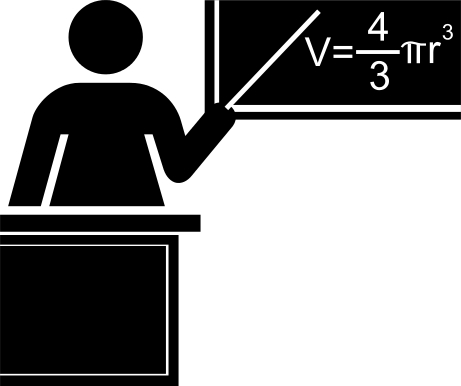
\includegraphics[width=.07\textwidth]{teacher.jpg} & 
\begin{minipage}{.85\textwidth}
}{%
\end{minipage}\\
\hline
\end{tabular}
}


%pour les fichiers c et dossiers
\newcounter{exoo} \setcounter{exoo}{0}
\newcommand{\numexo}{\theexoo}
\newcommand{\repexo}{{\tt exo\_\numexo}}
\newcommand{\exoplus}{\addtocounter{exoo}{1}}




\begin{document}
\maketitle





\thispagestyle{empty}

%\includegraphics

\begin{icone}{lecture.jpg}
    {\bf Ce symbole indique un texte à lire attentivement avant de se lancer dans les exercices qui suivent.}

    bla
\end{icone}

\section{Notion de script}




\section{Next}

\begin{icone}{sacoche.png}
    {\bf Ce symbole précise les compétences SACoche liées aux exercices qui suivent.}

    \bigskip

    {\sc type}
\end{icone} 

\bigskip

\begin{action}
\item Dans le mode console : définissez deux variables $a$ et $b$ valant respectivement 10 et 3, calculez ce que valent $a + b$, $a * b$ ou $a/b$. Changez la valeur de $b$ en $3.0$ et recommencez. Quelle est la différence ?
\item Toujours dans le mode console, utilisez la fonction {\tt type} pour demandez le type des objets. Créez des variables entières, des réels, des chaînes de caractères et affichez leur type.
\item Affichez maintenant une phrase mélangeant une chaîne de caractère et la valeur d'une variable.
\end{action}

\bigskip

\begin{icone}{lecture.jpg}
À partir de maintenant les exercices seront à traiter en écrivant des scripts (ou programmes) python. N'hésitez pas à revoir les vidéos correspondantes si nécessaire. N'oubliez pas d'ajouter la ligne

{    \tt \#coding: utf-8}

au début du programme si vous n'utilisez pas que des caractères ascii (accents, etc.)
\end{icone}


\begin{action}
\item \'Ecrivez un programme {\it age.py} qui demande son âge à l'utilisateur et répond en utilisant sa réponse au milieu d'une phrase, comme par exemple en lui donnant l'âge qu'il aura en 2027 (ou sinon, soyez imaginatifs, c'est vous les jeunes :) )
\item \'Ecrivez {\tt matieres.py} : demandez maintenant deux informations à l'utilisateur, sous forme de chaînes de caractères, et faites une phrase avec les deux informations. Par exemple, on lui demande le nom de ses deux matières préférées, et on répond "moi aussi j'adore (...) et (...) ."  ({\small Réponse : programmation et algorithmique}). {\it Attention à bien différencier les fonctions natives {\tt input} qui renvoie une {\it valeur} et {\tt raw\_input} qui renvoie une chaîne de caractères.}
\item Dans {\tt queltype.py}, demandez à l'utilisateur d'entrer une valeur avec {\tt input}, stockez la dans une variable et affichez son type. Rappel : {\tt type(a)} renvoie le type d'une variable a. Vous pouvez l'afficher avec {\tt print}. Testez avec différentes valeurs : {\tt 35, 284736537, -35, 2.4, -10.6, "bonjour", "b", [2,4,3], ["bonjour, "au revoir"], ...} . regardez bien le type à chaque fois.

\item Dans {\tt affichages.py}, affichez (sans utiliser de boucle) :
    \begin{itemize}
        \item la chaîne "aaaaaa..." (250 "a")
        \item la chaîne "bbbb....a" (250 "b" suivis d'un "a")
        \item la chaîne "bbbb....aaabbb..." (250 "b" suivis d'un "a" suivis de 100 b)
        \item La liste [0,1,...1000] (au complet)
        \item La liste [1000,1001,...1507] (au complet)
        \item 50 fois "bonjour" en allant à la ligne à chaque fois (utilisez "\textbackslash n")
    \end{itemize}

\end{action}

\newpage
\section{Les boucles}

\begin{icone}{youtube.jpg}
    La boucle {\tt while} en python

    La boucle {\tt for} en python
\end{icone}

\bigskip

\begin{icone}{tuto.jpg}
Partie 4 du tutoriel :

\url{https://docs.python.org/fr/2.7/tutorial/controlflow.html}
\end{icone}


\bigskip

\begin{icone}{sacoche.png}
{\sc BOUCLES1, BOUCLES2, BOUCLES?}\\
\end{icone} 

\bigskip




\begin{action}
\item \'Ecrire un programme qui affiche 50 fois "bonjour", cette fois-ci en utilisant une boucle {\tt while}.
\item Même exercice avec une boucle {\tt for}.
\item \'Ecrire un programme qui demande un mot et un entier, et affiche autant de fois le mot entré. Attention à distinguer {\tt raw\_input} et {\tt input}.
\item \'Ecrire un programme qui affiche un rectangle d'étoiles de p lignes et q colonnes. Par exemple si on entre 3 pour p et 12 pour q, la sortie sera: 
    \begin{lstlisting}
    *************
    *************
    *************
    \end{lstlisting}

\item \'Ecrire un programme qui affiche un triangle d'étoiles de taille donnée, par exemple si on entre $6$ le programme affiche :

    \begin{lstlisting}
    *
    **
    ***
    ****
    *****
    ******
    \end{lstlisting}

\item Même exercice mais cette fois la sortie est 

    \begin{tabular}{cccccc}
        & & & & &*\\
        & & & &*&* \\
        & & &*&*&* \\
        & &*&*&*&* \\
        &*&*&*&*&* \\
        *&*&*&*&*&* \\
    \end{tabular}
\end{action}

\end{document}
